\documentclass[output=paper]{langsci/langscibook}

\author{Kyle Johnson\affiliation{University of Massachusetts, Amherst}}
\title{Rethinking Linearization}

% \chapterDOI{} %will be filled in at production

\abstract{The reason \enquote{movement} is used to describe the relationship
    between an interrogative phrase in English and the syntactic position is
    binds a variable in, is because that variable is silent.
    Impressionistically, the interrogative phrase has changed location – it has
    moved from the position interpreted as a variable. To derive this feature
    of the relationship while maintaining a semantics that correctly captures
    the nature of the variable is not trivial. The presently best model is one
    that claims that the interrogative phrase is, at least partially, in both
    positions – the position it is spoken in and the position the variable is
    in. Jairo Nunes has suggested a method of using that model and an algorithm
    that converts syntactic representations into strings – a linearization
    algorithm – to derive the fact that a change of location is how being in
    two positions is manifest. I develop this idea in a framework that
    expresses the \enquote{be in two positions} syntax with phrase markers\is{phrase marker} that
allow a term to be dominated by more than one mother. This interpretation of
movement does not fit well with the execution Jairo Nunes had of his idea.  I
develop an alternative implementation that preserves his leading idea.}

\maketitle

\begin{document}\glsresetall

\section{Introduction}

In a series of papers, a book, and a dissertation, Jairo \citeauthor{Nunes1995}
has provided a compelling way of deriving a signature property of \isi{movement}, a
property I will call ``terseness.'' \nocite{Nunes1995, Nunes1996, Nunes1999}
\nocite{Nunes2004}

\begin{exe}
	\ex \label{ex:terseness} Terseness\\
    When a term is moved from one position to another, it gets spoken in only
    one of those positions.
\end{exe}

There are exceptions to Terseness, and some of these Nunes' account predicts.
This venue doesn't provide the space to consider these exceptions, or how they
fit Nunes' project, so I will set them aside and concentrate on the normal
case, in which Terseness holds. Nunes' leading idea is that \isi{movement} creates a
structure that the \isi{linearization} algorithm can interpret only if Terseness
holds.

Nunes' account has two parts. First, he adopts the Copy\is{copy theory of
movement} Theory of
Movement~(\ref{ex:ctm}).
\begin{exe}
	\ex \label{ex:ctm} Copy Theory of Movement
	\begin{xlist}
		\ex From a term X is made a copy: X$'$
		\ex X$'$ is merged into a position higher than X
	\end{xlist}
\end{exe}

On this view, \isi{movement} could take the structure in (\ref{ex:ds}), form a
copy\is{copy theory of movement} of \emph{which flower} and form the structure
in~(4).\footnote{In order to focus on just one \isi{movement} operation at a time, I
    will only consider cases of embedded constituent questions, where \isi{movement}
of the \obar{T} to \obar{C} doesn't occur.} %

\noindent\begin{minipage}[t]{.48\textwidth}
\ea\label{ex:ds}
    \hspace*{-2.5em}\begin{tikzpicture}[baseline, scale=.8]

        \Tree 	[.CP
                    C$^0$
                    [.TP
                        [.DP$\dag$
                            [.D$^{0}\dag$ she ]
                        ]
                        [.TP$\dag$
                            [.T$^0$ should ]
                            [.VP
                                [.V$^0$ bring ]
                                [.DP
                                    [.D$^0$ which ]
                                    [.NP
                                        [.N$^0$ flower ]
                                    ]
                                ]
                            ]
                        ]
                    ]
                ]

    \end{tikzpicture}
\z
\end{minipage}
\begin{minipage}[t]{.6\textwidth}
\ea
    \hspace*{-6em}\begin{tikzpicture}[baseline, scale=.8]

        \Tree   [.CP
                    [.DP$'$
                        [.D$^{0}$$'$
                            which$'$
                        ]
                        [.NP$'$
                            [.N$^{0}$$'$ flower$'$ ]
                        ]
                    ]
                    [.CP$\dag$
                        C$^0$
                        [.TP
                            [.DP$\dag$
                                [.D$^{0}\dag$ she ]
                            ]
                            [.TP$\dag$
                                [.T$^0$ should ]
                                [.VP
                                    [.V$^0$ bring ]
                                    [.DP
                                        [.D$^0$ which ]
                                        [.NP
                                            [.N$^0$ flower ]
                                        ]
                                    ]
                                ]
                            ]
                        ]
                    ]
                ]

    \end{tikzpicture}
\z
\end{minipage}

%\begin{exe}
%	\ex \label{ex:ds}
%	\small
%	\hspace*{-15pt}
%	\jtree
%	\! = {CP} <left>[xunit=2em]!left ^<right>[xunit=2em]!right .
%	\!left =
%		{\obar{C}}
%		.
%	\!right =
%		{TP}
%		:[xunit=2.5em]{DP$\dag$}(<vert>{\obar{D}$\dag$}(<vert>{she})) [xunit=2.5em]{TP$\dag$}
%		:[xunit=2.5em]{\obar{T}}(<vert>{should}) [xunit=2.5em]{VP}
%		:[xunit=2em]{\obar{V}}(<vert>{bring}) [xunit=2em]{DP}
%		:[xunit=1.5em]{\obar{D}}(<vert>{which}) [xunit=1.5em]{NP}<vert>{\obar{N}}<vert>{flower}
%		.
%	\endjtree
%	\hspace*{-40pt}
%	(4)
%	\small
%	\jtree
%	\! = {CP} <left>[xunit=3em]!left ^<right>[xunit=3em]!right .
%	\!left =
%		{DP$'$}
%		:[xunit=1.5em]{\obar{D}$'$}(<vert>{which$'$}) [xunit=1.5em]{NP$'$}<vert>{\obar{N}$'$}<vert>{flower$'$}
%		.
%	\!right =
%		{CP$\dag$}
%		:[xunit=2em]{\obar{C}} [xunit=2em]{TP}
%		:[xunit=2.5em]{DP$\dag$}(<vert>{\obar{D}$\dag$}(<vert>{she})) [xunit=2.5em]{TP$\dag$}
%		:[xunit=2.5em]{\obar{T}}(<vert>{should}) [xunit=2.5em]{VP}
%		:[xunit=2.5em]{\obar{V}}(<vert>{bring}) [xunit=2.5em]{DP}
%		:[xunit=1.5em]{\obar{D}}(<vert>{which}) [xunit=1.5em]{NP}<vert>{\obar{N}}<vert>{flower}
%		.
%	\endjtree
%\end{exe}

The second part relies on a standard condition on how phrase markers\is{phrase marker} are
linearized into strings that \cite{Kayne1994} calls Antisymmetry.

\begin{exe}
	\ex \label{ex:antisymm} Antisymmetry\\
	A \isi{linearization} cannot contain both $a<b$ and $b<a$.
\end{exe}

Antisymmetry assumes that a \isi{linearization} is a set of ordered pairs $x<y$,
where $x$ and $y$ are words and ``<'' is the precedence relation. Antisymmetry
simply states that no word can both follow and precede another. Nunes' second
proposal, then, is that Antisymmetry cannot distinguish one word from .
The structure in (4) is not pronounced with two instances of \emph{which} and
\emph{flower} because a \isi{linearization} that contains both
\emph{which$'$}<\emph{she} and \emph{she}<\emph{which} will be a violation of
Antisymmetry. This is Terseness.

One goal of this paper is to define copies so that they have the effect of
invoking Antisymmetry in the way that Nunes envisions. That definition will use
the idea broached in \cite{Engdahl1980} that a moved term is a term in two
syntactic positions.\footnote{Engdahl cites the unpublished \citet{PetRit1981}
as her source for the idea.} This can be represented by letting \isi{phrase marker}
trees allow \isi{multidominance}. Another goal of this paper is to devise a
linearization algorithm that can handle such trees.

\section{Nunes' Proposal} % (fold)
\label{sec:nunesproposal}

Nunes couches his idea with a slightly modified version of the linearization
algorithm in \cite{Kayne1994}. The key departure from Kayne's algorithm
concerns the items that are linearized. Kayne's algorithm linearizes morphemes
-- including subword material -- and Nunes' doesn't. I'll adopt Nunes' view,
which is useful in accounting for certain exceptions to Terseness. A goal of
Kayne's work is to derive (\ref{ex:precede}) from the \isi{linearization} algorithm.
\begin{exe}
	\ex \label{ex:precede}
    If XP asymmetrically c-commands YP, then the words dominated by XP (=d(XP))
    will precede the words dominated by YP (=d(YP)) (modulo the effects of
    \isi{movement}).
    \ex α c-commands β if every phrase dominating α dominates β too, and α
    doesn't dominate β. α asymmetrically c-commands β if α c-commands β and β
    doesn't c-command α.
\end{exe}

This is achieved by building (\ref{ex:precede}) into the linearization
algorithm along the lines of~(\ref{ex:lca1}).
\begin{exe}
	\ex \label{ex:lca1}
	\begin{xlist}
		\ex Let $L$ be the set of pairs of heads and phrases, <$A,B$>, in a \isi{phrase marker} P such that $A$ asymmetrically c-commands $B$.
		\ex The \isi{linearization} of P is the union of d($A$) < d($B$) for every <$A,B$> in~$L$.%
		\footnote{More explicitly: the \isi{linearization} of P is \{$a<b$: $\forall a \in d(A)$ and $\forall b \in d(B)$ if <$A,B$> is in $L$ of P\}. Note that ``<'' is the precedes relation.} %
	\end{xlist}
\end{exe}

As Kayne notes, (\ref{ex:lca1}) needs to be weakened if it is to work for
phrase markers that have Specifiers. To see this, consider how (\ref{ex:lca1})
applies to~(\ref{ex:specill1}).
\ea\label{ex:specill1}
    \begin{tikzpicture}[baseline]

        \Tree 	[.TP
                    [.DP
                        [.D$^0$ the ]
                        [.NP
                            [.N$^0$ child ]
                        ]
                    ]
                    [.TP$\dag$
                        [.T$^0$ will ]
                        [.VP
                            [.V$^0$ cry ]
                        ]
                    ]
                ]

    \end{tikzpicture}
\z
%\begin{exe}
%	\ex \label{ex:specill1}
%	\jtree
%	\! = {TP} <left>[xunit=2.5em]!left ^<right>[xunit=2.5em]!right .
%	\!left =
%		{DP}
%		:[xunit=1.5em]{\obar{D}}(<vert>{the}) [xunit=1.5em]{NP}<vert>{\obar{N}}<vert>{child}
%		.
%	\!right =
%		{TP$\dag$}
%		:[xunit=1.5em]{\obar{T}}(<vert>{will}) [xunit=1.5em]{VP}<vert>{\obar{V}}<vert>{cry}
%		.
%	\endjtree
%\end{exe}

The $L$ for (\ref{ex:specill1}) is (\ref{ex:specill1L}), and this produces the
linearization in~(\ref{ex:specill1LL}).

\begin{exe}
	\ex \label{ex:sill1}
	\begin{xlist}
		\ex \label{ex:specill1L} $L$ = \parbox[t]{4in}{<\obar{D},\obar{N}>, <DP,\obar{T}>, <DP,VP>, <DP,\obar{V}>, <\obar{T},\obar{V}>, <TP$\dag$,\obar{D}>, <TP$\dag$,\obar{N}>}
		\medskip
		\ex \label{ex:specill1LL}
		$\left\{
		% \text{%\small
			\begin{array}{lll}
				the < child	&	child < can & can < cry\\
				the < can		&	child < cry\\
				the < cry		&							& can < the\\
										&							& cry < the\\
										&							& can < child\\
										&							& cry < child
			\end{array}
			% }
		\right\}$\\[5pt]
		$\equiv$ can cry the child can cry
	\end{xlist}
\end{exe}

(\ref{ex:specill1LL}) violates Antisymmetry.
\begin{exe}
	\ex \label{ex:antisymmb} Antisymmetry\\
	A \isi{linearization} cannot contain both $a$<$b$ and $b$<$a$.
\end{exe}

The problem with (\ref{ex:lca1}) is that it allows too many asymmetric
c-commanding pairs to enter $L$. Because TP$\dag$ is part of some of the pairs
in $L$, the orderings \emph{can<the}, \emph{can<child}, \emph{cry<the} and
\emph{cry<child} get into the \isi{linearization}. But because DP is also part of
some of the pairs in $L$, the \isi{linearization} contains \emph{the<can},
\emph{the<cry}, \emph{child<can} and \emph{child<cry}. To address this problem,
Kayne proposes a way of limiting the class of items that can be in $L$ so that
it achieves certain goals his system has for ordering sub-word morphemes.
Because that is not a feature of the procedure needed to derive Terseness, I
will take a slightly different tack. I will limit $L$ to just maximal and
minimal projections.
\begin{exe}
	\ex \label{ex:lca2}
	\begin{xlist}
		\ex Let $L$ be the set of pairs of heads and maximal projections, <$A,B$>, in a \isi{phrase marker} P such that $A$ asymmetrically c-commands $B$.
		\ex The \isi{linearization} of P is the union of d($A$) < d($B$) for every ordered pair in~$L$.
	\end{xlist}
\end{exe}

Because TP$\dag$ is neither a minimal nor a maximal projection it will be
jettisoned from $L$. (\ref{ex:lca2}) will produce the $L$ in
(\ref{ex:specill2L}), and this generates the correct linearization
in~(\ref{ex:specill2LL}).
\begin{exe}
	\ex \label{ex:sill2}
	\begin{xlist}
		\ex \label{ex:specill2L}
		$L$ = \parbox[t]{4in}{<\obar{D},\obar{N}>, <DP,\obar{T}> <DP,VP>, <DP,\obar{V}>, <\obar{T},\obar{V}>}
				\medskip
				\ex \label{ex:specill2LL}
				$\left\{
				% \text{%\small
					\begin{array}{lll}
						the < child	&	child < can & can < cry\\
						the < can		&	child < cry\\
						the < cry		&
					\end{array}
					% }
				\right\}$\\[5pt]
				$\equiv$ the child can cry
	\end{xlist}
\end{exe}

(\ref{ex:lca2}) correctly linearizes a wide array of syntactic structures and
provides a way of deriving~(\ref{ex:precede}).

We are now ready to see how Nunes proposes to derive Terseness. His proposal
amounts to adopting~(\ref{ex:defcopy}).
\begin{exe}
	\ex \label{ex:defcopy}
	A term, X, and , X$'$, cannot be distinguished by Antisymmetry.
\end{exe}

A consequence of (\ref{ex:defcopy}) is that a \isi{linearization} which contains both
X<Y and Y<X$'$ will violate Antisymmetry. Applying (\ref{ex:lca2}) to the
result of \isi{movement} in (4) produces the \isi{linearization} in~(\ref{ex:dslin}b).
\begin{exe}
	\ex \label{ex:dslin}
	\begin{xlist}
		\small
	\ex $L$ = \parbox[t]{4in}{<\obar{D}$'$,\obar{N}$'$>, <DP$'$,\obar{C}>, <DP$'$,TP>, <DP$'$,DP$\dag$>, <DP$'$,\obar{D}$\dag$>, <DP$'$,\obar{T}>, <DP$'$,VP>, <DP$'$,\obar{V}>, <DP$'$,DP>, <DP$'$,\obar{D}>, <DP$'$,NP>, <DP$'$,\obar{N}>, <\obar{C},DP$\dag$>, <\obar{C},\obar{D}$\dag$>, <\obar{C},\obar{T}>, <\obar{C},VP>, <\obar{C},\obar{V}>, <\obar{C},DP>, <\obar{C},\obar{D}>, <\obar{C},NP>, <\obar{C},\obar{N}>, <DP$\dag$,\obar{T}>, <DP$\dag$,VP>, <DP$\dag$,\obar{V}>, <DP$\dag$,DP>, <DP$\dag$,\obar{D}>, <DP$\dag$,NP>, <DP$\dag$,\obar{N}>, <\obar{T},\obar{V}>, <\obar{T},DP>, <\obar{T},\obar{D}>, <\obar{T},NP>, <\obar{T},\obar{N}>, <\obar{V},\obar{D}>, <\obar{V},NP>, <\obar{V},\obar{N}>, <\obar{D},\obar{N}>}

	\ex \
	\linebreak

	\hspace*{-20pt}
	\footnotesize
	$\left\{
		\begin{array}{llllll}
            \text{\emph{which$'$ < flower$'$}} & \text{\emph{flower$'$ < should}} & \text{\emph{should < she}}      & \text{\emph{she < bring}}  & \text{\emph{bring < which}}\\% & which < flower\\
            \text{\emph{which$'$ < should$'$}} & \text{\emph{flower$'$ < she}} & \text{\emph{should < bring}}    & \text{\emph{she < which}}  & \text{\emph{bring < flower}}\\
            \text{\emph{which$'$ < she}}     & \text{\emph{flower$'$ < bring}} & \text{\emph{should < which}}    & \text{\emph{she < flower}} & \text{\emph{which < flower}}\\
            \text{\emph{which$'$ < bring}}   & \text{\emph{flower$'$ < which}}     & \text{\emph{should < flower}}\\
            \text{\emph{which$'$ < which}}   & \text{\emph{flower$'$ < flower}} \\
            \text{\emph{which$'$ < flower}}
    \end{array}
    \right\}$\\[5pt] \normalsize
	$\equiv$ which$'$ flower$'$ should she bring which flower
	\end{xlist}
\end{exe}

Because of the existence of \emph{which'<bring} and \emph{bring<which} in
(\ref{ex:dslin}b), along with many other such pairs, Antisymmetry is violated.

This derives the impossibility of speaking a moved term in both of the places
it occupies, but something more is needed to produce the string that actually
arises. Nunes suggests that this involves a movement-specific deletion
operation which removes orderings from a \isi{linearization}. Applied to
(\ref{ex:dslin}), this deletion operation could remove orderings to form one of
the strings in (\ref{ex:fixeddslin}), all of which satisfy Antisymmetry.
\begin{exe}
	\ex \label{ex:fixeddslin}
	\begin{xlist}
		\ex which flower should she bring
		\ex which should she bring flower
		\ex flower should she bring which
		\ex should she bring which flower
	\end{xlist}
\end{exe}

Nunes assumes, and so shall I, that (\ref{ex:fixeddslin}a) and
(\ref{ex:fixeddslin}d) are possible outcomes -- some languages choosing one or
the other -- but that (\ref{ex:fixeddslin}b) and (\ref{ex:fixeddslin}c) are
not. To block these two outcomes, Nunes makes two assumptions. First the
deletion operation in question applies not to a \isi{linearization} -- it doesn't
remove elements of the set in (\ref{ex:dslin}) for instance -- but to the
syntactic structure being linearized. It removes the \isi{linearization} statements
corresponding to the phrases and heads that populate a syntactic
representation. I'll formulate Nunes' condition, which he calls Chain
Reduction, to reflect this.
\begin{exe}
	\ex \label{ex:chain} Chain Reduction\\
	Chain Reduction applied to d(X) deletes every ordered pair in a \isi{linearization} that contains a word in d(X), X a head or phrase.
\end{exe}

To form the strings in (\ref{ex:fixeddslin}), Chain Reduction will delete from $L$ the ordered pairs indicated in~(\ref{ex:crill1}).
\begin{exe}
	\ex \label{ex:crill1}
	\begin{xlist}
		\ex To form (\ref{ex:fixeddslin}a), Chain Reduction applies to d(DP).
		\ex To form (\ref{ex:fixeddslin}b), Chain Reduction applies to d(NP$'$) and d(\obar{D}).
		\ex To form (\ref{ex:fixeddslin}c), Chain Reduction applies to d(\obar{D}') and d(NP).
		\ex To form (\ref{ex:fixeddslin}a), Chain Reduction applies to d(DP').
	\end{xlist}
\end{exe}

The second assumption Nunes makes is that there is an economy condition that favors fewer targets for Chain Reduction.
\begin{exe}
	\ex \label{ex:econ} Economy\\
	Let $N$ be the number of terms that an instance of Chain Reduction, $R$, applies to. Block $R$ if its $N$ is greater than the $N$ for another $R$ that satisfies Antisymmetry.
\end{exe}

Economy will block the applications of Chain Reduction in (\ref{ex:crill1}b) and (\ref{ex:crill1}c) because of the equally Antisymmetry compliant applications of Chain reduction in (\ref{ex:crill1}a) and~(\ref{ex:crill1}d).

There are a variety of successes for this method of deriving Terseness, and I
will not challenge it. Instead, I will focus on understanding
(\ref{ex:defcopy}). Why is Antisymmetry unable to distinguish a term from its
copy?\is{copy theory of movement}

% section nunesproposal (end)

\section{Multidominance} % (fold)
\label{sec:multidominance}

A simple way of explaining why a term and  are the same thing for Antisymmetry
is that they \emph{are} the same thing. Rather than modeling \isi{movement} as an
operation that creates a copy\is{copy theory of movement} of a term and puts
that term in an additional position, we could model \isi{movement} as an operation
that puts one term in two positions. This is a thesis that \citet{Engdahl1980},
\citet{Starke2001}, \citet{deVries2007}, \citet{Gartner2002}, among others,
have suggested.

An immediate problem with this view, though, is that it leads to the
expectation that the denotation a phrase has will be the same in both of the
positions \isi{movement} relates it to. Consider, for instance, a way of representing
this thesis that allows one term to have two positions in a \isi{phrase marker}. That
would give (4) the representation in~(\ref{ex:multi1}).\largerpage

\ea\label{ex:multi1}
    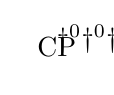
\begin{tikzpicture}[baseline, scale=.95]
        \tikzset{level 1/.style={sibling distance=-80pt}}
        \Tree   [.\node(cp){CP};
                    [.CP$\dag$
                        C$^0$
                        [.TP
                            [.DP$\dag$
                                [.D$^{0}\dag$ she ]
                            ]
                            [.TP$\dag$
                                [.T$^0$ should ]
                                [.VP
                                    [.V$^0$ bring ]
                                    [.\node(dp){DP};
                                        [.D$^0$ which ]
                                        [.NP
                                            [.N$^0$ flower ]
                                        ]
                                    ]
                                ]
                            ]
                        ]
                    ]
                    \edge [draw=none]; {}
                ]

            \draw [bend left=40] (cp.south) to (dp.north);
    \end{tikzpicture}
\z
%
%\begin{exe}
%	\ex \label{ex:multi1}
%	\small
%	\jtree
%	\! = {CP}@r  <left>[xunit=2.5em]!left .
%	\!left =
%		{CP$\dag$}
%		:[xunit=2.6em]{\obar{C}} [xunit=2.5em]{TP}
%		:[xunit=2.5em]{DP$\dag$}(<vert>{\obar{D}$\dag$}(<vert>{she})) [xunit=2.5em]{TP$\dag$}
%		:[xunit=2.7em]{\obar{T}}(<vert>{should}) [xunit=2.7em]{VP}
%		:[xunit=2.5em]{\obar{V}}(<vert>{bring}) [xunit=2.5em]{DP}@s
%		:[xunit=1.5em]{\obar{D}}(<vert>{which}) [xunit=1.5em]{NP}<vert>{\obar{N}}<vert>{flower}
%		.
%		\nccurve[dirA=(1:-1),dirB=(.1:1)]{-}{r:b}{s:t}
%	\endjtree
%\end{exe}

There is evidence that the semantics of constituent questions of this kind must be able to involve a binder/variable relation. In principle, we want phrasal \isi{movement} to be able to cause a moved phrase to bind a variable in the position it moves from. The representation in (\ref{ex:multi1}) makes that possibility obscure. The single phrase, \emph{which flower}, would not seem to be able to simultaneously have the meaning of a variable and the meaning of the term that binds that variable.%
\footnote{But see \cite{Engdahl1986} for a method.} %
We want to define ``copy of'' so that it gives the equivalent of (\ref{ex:multi1}) for Antisymmetry, but not for the meanings involved.

In \cite{Johnson2012}, I argue that the solution to this dilemma comes from
recognizing that there can be material in the higher position that is not part
of the term that has moved. If we represent this additional material with
``Q,'' then (\ref{ex:multi1}) can be replaced by~(\ref{ex:multi2}).

\ea\label{ex:multi2}
    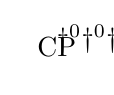
\begin{tikzpicture}[baseline]
        \tikzset{level 1/.style={sibling distance=-80pt}}
        \Tree   [.\node(cp){CP};
                    [.CP$\dag$
                        C$^0$
                        [.TP
                            [.DP$\dag$
                                [.D$^{0}\dag$ she ]
                            ]
                            [.TP$\dag$
                                [.T$^0$ should ]
                                [.VP
                                    [.V$^0$ bring ]
                                    [.\node(dp){DP};
                                        [.D$^0$ which ]
                                        [.NP
                                            [.N$^0$ flower ]
                                        ]
                                    ]
                                ]
                            ]
                        ]
                    ]
                    [.\node(xp){XP};
                        [.X$^0$ Q ]
                        \edge [draw=none]; {}
                    ]
                ]

            \draw [bend left=40] (xp.south) to (dp.north);
    \end{tikzpicture}
\z
%
%\begin{exe}
%	\ex \label{ex:multi2}
%	\small
%	\jtree
%	\! = {CP} <left>[xunit=4.5em]!left ^<right>[xunit=6em]!right .
%	\!left =
%		{CP$\dag$}
%		:[xunit=2.5em]{\obar{C}} [xunit=2.5em]{TP}
%		:[xunit=2.6em]{DP$\dag$}(<vert>{\obar{D}$\dag$}(<vert>{she})) [xunit=2.7em]{TP$\dag$}
%		:[xunit=2.5em]{\obar{T}}(<vert>{should}) [xunit=2.5em]{VP}
%		:[xunit=2.5em]{\obar{V}}(<vert>{bring}) [xunit=2.5em]{DP}@s
%		:[xunit=1.5em]{\obar{D}}(<vert>{which}) [xunit=1.5em]{NP}<vert>{\obar{N}}<vert>{flower}
%		.
%	\!right =
%		{XP}@r
%		<left>[xunit=2em]{\obar{X}}<vert>{Q}
%		.
%		\nccurve[dirA=(1:-1),dirB=(.8:1)]{-}{r:b}{s:t}
%	\endjtree
%\end{exe}

Depending on the kind of semantic relation involved, we can credit the
denotation of \obar{Q} with being responsible for creating a binder out of the
higher phrase. See \cite{Johnson2012} for details. I will assume that \isi{movement}
is an operation that puts one term in two positions, but that it does so always
in a way parallel to (\ref{ex:multi2}). The moved item is part of a larger term
in the higher position.

Adopting this view requires a recasting of Nunes' method of deriving Terseness.
We cannot rely on an operation like Chain Reduction to fix the violations of
Antisymmetry that \isi{movement} will create as it will overshoot. To see this,
consider how (\ref{ex:lca2}) will apply to~(\ref{ex:multi2}); it produces the
linearization in~(\ref{ex:multi2lcad}).
\begin{exe}
	\ex \label{ex:multi2lcad}
	\begin{xlist}
		\small
        \ex $L$ = \parbox[t]{4in}{<\obar{X},\obar{D}>, <\obar{X},NP>,
        <\obar{X},\obar{N}>, <XP,\obar{C}>, <XP,\obar{C}>, <XP,TP>,
    <XP,DP$\dag$>, <XP,\obar{D}$\dag$>, <XP,\obar{T}>, <XP,VP>, <XP,\obar{V}>,
<\obar{C},DP$\dag$>, <\obar{C},\obar{D}$\dag$>, <\obar{C},VP>,
<\obar{C},\obar{V}>, <\obar{C},DP>, <\obar{C},\obar{D}>, <\obar{C},NP>,
<\obar{C},\obar{N}>, <DP$\dag$,\obar{T}>, <DP$\dag$,VP>, <DP$\dag$,\obar{V}>,
<DP$\dag$,DP>, <DP$\dag$,\obar{D}>, <DP$\dag$,NP>, <DP$\dag$,\obar{N}>,
<\obar{T},\obar{V}>, <\obar{T},DP>, <\obar{T},\obar{D}>, <\obar{T},NP>,
<\obar{T},\obar{N}>, <\obar{V},\obar{D}>, <\obar{V},NP>, <\obar{V},\obar{N}>,
<\obar{D}, \obar{N}>}\\[1em]
		\ex
		%\linebreak
		\hspace*{-5pt}
		\footnotesize
		$\left\{
			\begin{array}{llllll}
%			Q < which & which < flower & flower < she & she < should & should < bring & bring < which\\
%			Q < flower & which < she & flower < should & she < bring & should < which & bring < flower\\
%			Q < she & which < should & flower < bring & she < which & should < flower\\
%			Q < should    & which < bring & flower < which & she < flower\\
%			Q < bring &  which < which & flower < flower\\
\text{\emph{Q < which  }} & \text{\emph{which < flower}} & \text{\emph{flower < she}}    & \text{\emph{she < should  }} & \text{\emph{should < bring}} \\% &  \\
\text{\emph{Q < flower }} & \text{\emph{which < she   }} & \text{\emph{flower < should}}  & \text{\emph{she < bring   }} & \text{\emph{should < which}} \\%   & \\
\text{\emph{Q < she    }} & \text{\emph{which < should}} & \text{\emph{flower < bring }} & \text{\emph{she < which   }} & \text{\emph{should < flower}} \\
\text{\emph{Q < should }} & \text{\emph{which < bring }} & \text{\emph{flower < which }} & \text{\emph{she < flower}} & \text{\emph{bring < which}} \\
\text{\emph{Q < bring  }} & \text{\emph{which < which }} & \text{\emph{flower < flower}} &                            &  \text{\emph{bring < flower}} \\
			\end{array}
		\right\}$\\[5pt]
		\normalsize
		$\equiv$ Q which flower should she bring which flower
	\end{xlist}
\end{exe}

There are numerous violations of Antisymmetry in (\ref{ex:multi2lcad}b) (e.g.,
\emph{which<bring} and \emph{bring<which}) as well as the arguably anomalous
\emph{which<which} and \emph{flower<flower}. For Chain Reduction to remove
these violations, it would have to apply to either d(XP) or d(DP). If it
applies to d(DP), (\ref{ex:multi2lcad}) will lose all ordered pairs that have
either \emph{which} or \emph{flower} in them, producing a \isi{linearization} that is
equivalent to~(\ref{ex:multi2tool}).

\begin{exe}
	\ex \label{ex:multi2tool}
	Q she should bring
\end{exe}

If \isi{movement} puts one thing in two places, thereby explaining (\ref{ex:defcopy}), then something must replace Chain Reduction in Nunes' explanation for Terseness.

A minimal modification of Nunes' system would be to allow the pairs that go into $L$ to be partial in a way that mimics Chain Reduction. Rather than removing ordering statements that produce a violation of Antisymmetry, we can allow the \isi{linearization} to avoid introducing them to begin with. (\ref{ex:lca2}) becomes~(\ref{ex:lca3}).
\begin{exe}
	\ex \label{ex:lca3}
	\begin{xlist}
		\ex Let $L$ be a set of pairs of heads and maximal projections, <$A,B$>, in a \isi{phrase marker} P such that $A$ asymmetrically c-commands $B$.
		\ex The \isi{linearization} of P is the union of d($A$) < d($B$) for every ordered pair in~$L$.
	\end{xlist}
\end{exe}

Unlike (\ref{ex:lca2}a), which required that $L$ contain <$A,B$> for every $A$
that asymmetrically c-commands $B$, (\ref{ex:lca3}a) allows $L$ to contain a
proper subset of such ordered pairs: all it requires is that $L$ contain
<$A,B$> only if $A$ asymmetrically c-commands~$B$. (\ref{ex:lca3}) allows
partial orderings, and so it will have to be coupled with something that
ensures that every word in a syntactic representation end up in the
linearization. This can be achieved by adopting another of \citegen{Kayne1994}'s
well-formedness conditions:

\begin{exe}
	\ex \label{ex:totality} Totality\\
	If $a$ and $b$ are words in P, then either $a<b$ or $b<a$ must be in the \isi{linearization} of~P.
\end{exe}

(\ref{ex:lca3}) will allow for the English \isi{linearization} of (\ref{ex:multi2}) -- in (\ref{ex:multi2lca3d}) -- and Totality will prevent incomplete outcomes like~(\ref{ex:multi2tool}).
\begin{exe}
	\ex \label{ex:multi2lca3d}
	\begin{xlist}
		\small
			\ex $L$ = \parbox[t]{4in}{<\obar{X}, \obar{D}>, <\obar{X}, \obar{N}>, <\obar{D},\obar{N}>, <XP,\obar{C}>, <XP, DP$\dag$>, <XP,\obar{T}>, <XP,\obar{V}>, <\obar{C},DP$\dag$>, <\obar{C},\obar{T}>, <\obar{C}, \obar{V}>, <DP$\dag$,\obar{T}>, <DP$\dag$,\obar{V}>, <\obar{T},\obar{V}>}
			\ex %\
			%\linebreak
			\hspace*{-5pt}
			\footnotesize
			$\left\{
				\begin{array}{lllll}
%				Q < which & which < flower & flower < she & she < should & should < bring\\
%				Q < flower & which < she & flower < should & she < bring\\
%				Q < she & which < should & flower < bring\\
%				Q < should   & which < bring\\
%				Q < bring
\text{\emph{Q < which  }} & \text{\emph{which < flower}} & \text{\emph{flower < she}}    & \text{\emph{she < should}} & \text{\emph{should < bring}} \\% &  \\
\text{\emph{Q < flower }} & \text{\emph{which < she   }} & \text{\emph{flower < should}} & \text{\emph{she < bring }} \\%   & \\
\text{\emph{Q < she    }} & \text{\emph{which < should}} & \text{\emph{flower < bring }}                              \\
\text{\emph{Q < should }} & \text{\emph{which < bring }}                                                              \\
\text{\emph{Q < bring  }} &                                                                                           \\
				\end{array}
			\right\}$\\[5pt]
            \normalsize
			$\equiv$ Q which flower she should bring
	\end{xlist}
\end{exe}

Moreover, (\ref{ex:lca3}) will also correctly block (\ref{ex:fixeddslin}b) and
(\ref{ex:fixeddslin}c), in which \emph{which} and \emph{flower} are linearized
in non-contiguous positions. This is because for Totality to be satisfied, XP
must be in $L$. Only if XP is in $L$ will Q get linearized with all the words
that are not in XP. But once XP is in $L$, all of the words in XP (i.e.,
\emph{Q}, \emph{which} and \emph{flower}) will be linearized in the same way to
every word not in XP. A feature of (\ref{ex:lca3}) is that it enforces
contiguity on any phrase that enters~$L$.  \footnote{There is a very close
resemblance between Contiguity and the central condition in Lisa Selkirk's
Match Theory \citep{Selkirk2011}, which requires that phrases map onto
prosodic units that contain every word within them. A tantalizing prospect is
to reduce Contiguity to this condition on the syntax/prosody mapping.} %
\begin{exe}
	\ex \label{ex:contiguity} Contiguity\\
	A \isi{linearization} is contiguous if for every phrase, XP, in $L$, if $b$ $\notin$ d(XP), then $b<a$ or $a<b$ for every $a \in$ d(XP).
\end{exe}

An interesting feature of \isi{movement} is that it creates structures which violate
a stronger form of Contiguity, one that holds of every phrase in a structure,
not just those used to form a \isi{linearization}. This stronger form of Contiguity
is quite widely honored by linearization; we should have an account for why it
is relaxed just for \isi{movement} structures. (\ref{ex:lca3}) takes a step towards
doing this by letting Contiguity hold not of the entire \isi{phrase marker}, but of
the subset of phrases chosen from that \isi{phrase marker} to base a linearization
on. Totality forces this subset to be sufficiently representative, spreading
Contiguity among the non-moved parts of the \isi{phrase marker}. The moved parts of a
phrase marker are allowed to violate Contiguity because there is a way of
satisfying Totality without considering all the positions they are in.

Unfortunately, this feature of (\ref{ex:lca3}) prevents any other linearization
of (\ref{ex:multi2}), including the one Nunes' theory countenanced
in~(\ref{ex:covert}).
\begin{exe}
	\ex \label{ex:covert} Q she should bring which flower
\end{exe}

In general, if phrasal \isi{movement} creates a structure in which, like
(\ref{ex:multi2}), the moved phrase is part of a larger phrase in the higher
position, then (\ref{ex:lca3}) will not allow covert \isi{movement}.

What this section shows is that it's possible to preserve much of the
linearization algorithm that Nunes uses to explain Terseness, while giving a
natural and simple explanation for why Antisymmetry should treat a moved term
as if it's one thing in two positions. Kayne called his \isi{linearization} algorithm
the \enquote{\glsunset{LCA}\glsdesc{LCA}}, or \gls{LCA}. Let's know this modified
version of his algorithm as the \enquote{\glsunset{MLCA}\glsdesc{MLCA}}, or
\gls{MLCA}.\is{Linear Correspondence Axiom}

\begin{exe}
    \ex \label{ex:mlca} \gls{MLCA}
	\begin{xlist}
		\ex Let $L$ of P consist of pairs of minimal and maximal projections, <$A,B$>, where $A$ asymmetrically c-commands $B$ in P.
		\ex A \isi{linearization} of P is the union of d($A$)<d($B$) for every <$A,B$> in $L$ of P.
        \ex d(α) =$_{def.}$ all the words dominated by α.
	\end{xlist}
	\ex Antisymmetry\\
	A \isi{linearization} of P cannot contain both $a<b$ and $b<a$.
	\ex Totality\\
	A \isi{linearization} of P must contain $a<b$ or $b<a$ for every pair of words $a,b$ in P.
\end{exe}

The \gls{MLCA} has properties which should be regarded as features. Some of them are~(\ref{ex:features}).
\begin{exe}
	\ex \label{ex:features} \gls{MLCA} Features
	\begin{xlist}
        \ex Preserves the goal of Kayne's \gls{LCA}, i.e. the generalization in (\ref{ex:precede}).
		\ex Enforces Contiguity on a moved phrase (i.e., blocks (\ref{ex:fixeddslin}b) and (\ref{ex:fixeddslin}c)).
		\ex Derives Terseness.
		\ex Produces linearizations corresponding to overt \isi{movement}.
	\end{xlist}
\end{exe}

It also has a property that could be regarded a bug. If \isi{movement} has the properties I argued for in \citet{Johnson2012}, then it will not allow for a \isi{linearization} that corresponds to covert \isi{movement}. I regard that as a bug, and so I will offer an alternative \isi{linearization} scheme in the next section.

% section \isi{multidominance} (end)

\section{Paths} % (fold)
\label{sec:paths}

If a structure like (\ref{ex:multi2}) is to be able to linearize into covert \isi{movement}, i.e. a string in which \emph{which flower} follows \emph{bring}, then it will be necessary to allow \emph{Q} and \emph{which flower} to end up non-contiguous. This means that the \isi{linearization} algorithm cannot prevent \emph{Q} from getting into the \isi{linearization} unless everything else in d(XP) gets ordered the same way to the things that XP asymmetrically c-commands. We must let \emph{Q} get into the \isi{linearization} without using XP's position to do so. I cannot see a way of doing that which preserves Kayne's program, so I will abandon (\ref{ex:precede}) as a goal of the \isi{linearization} scheme.%
\footnote{See \cite{AbeNee2012} for another direction to pursue.} %
What shouldn't be abandoned, though, is Contiguity which seems to be a general truth about how syntactic structures map onto strings. If \isi{movement} employs multidominant representations, Contiguity must be relaxed, but only just where \isi{multidominance} arises. So my goal will be to devise a \isi{linearization} algorithm which preserves Contiguity in all those cases where \isi{multidominance} (aka \isi{movement}) doesn't arise and explain why it selectively permits violations where \isi{multidominance} does arise.

Contiguity is typically conceived of as a relationship between dominance relations and contiguous strings and this is how I've stated it in (\ref{ex:contiguity}). It enforces the law in~(\ref{ex:contex1}).
\begin{exe}
	\ex \label{ex:contex1}
	If words $a_1$,\ldots,$a_n$ are dominated by a phrase XP (=d(XP)), then $a_1$,\ldots,$a_n$ will form a contiguous substring in the \isi{linearization}.
\end{exe}

For standard phrase markers\is{phrase marker} that don't have \isi{multidominance} in them, an equally valid way of stating the law that Contiguity enforces is~(\ref{ex:secondlaw}).
\begin{exe}
	\ex \label{ex:secondlaw}
	If phrase XP\tss{1} dominates phrase XP\tss{2}, then the words in XP\tss{2} (i.e., d(XP\tss{2})) will form a contiguous substring of the string formed by the words in XP\tss{1} (i.e., d(XP\tss{1})).
\end{exe}

Indeed, the transitive closure of (\ref{ex:secondlaw}) holds for phrase markers\is{phrase marker} that obey Contiguity and don't contain \isi{multidominance}.
\begin{exe}
	\ex \label{ex:thirdlaw}
	Let $p$=(XP\tss{1}, XP\tss{2},\ldots,XP\tss{n}) be a series of phrases such that every XP\tss{i} in $p$ is dominated by every XP$_{j \leq i}$ in $p$. For every $p$ in a \isi{phrase marker}, d(XP\tss{i}) must be a contiguous substring of d(XP$_{j \leq i}$) for every XP in $p$.\\[8pt]
	(NB: ``dominance'' and ``substring'' are reflexive.)
\end{exe}

I will call a series of phrases that form a $p$, a ``path.''

Interestingly, (\ref{ex:thirdlaw}) isn't obeyed in a phrase-marker that allows
for multidominant representations. To see this, consider~(\ref{ex:multi3}) and
the \isi{linearization} of (\ref{ex:multi3}) that corresponds to overt \isi{movement},
in~(\ref{ex:linmulti3}).

\ea\label{ex:multi3}
    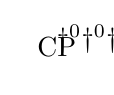
\begin{tikzpicture}[baseline]

        \tikzset{level 1/.style={sibling distance=-80pt}}
        \Tree   [.\node(cp){CP};
                    [.CP$\dag$
                        C$^0$
                        [.TP
                            [.DP$\dag$
                                [.D$^{0}\dag$ she ]
                            ]
                            [.TP$\dag$
                                [.T$^0$ should ]
                                [.VP
                                    [.VP$\dag$
                                        [.V$^0$ bring ]
                                        [.\node(dp){DP};
                                            [.D$^0$ which ]
                                            [.NP
                                                [.N$^0$ flower ]
                                            ]
                                        ]
                                    ]
                                    [.PP
                                        [.P$^0$ here ]
                                    ]
                                ]
                            ]
                        ]
                    ]
                    [.\node(xp){XP};
                        [.X$^0$ Q ]
                        \edge [draw=none]; {}
                    ]
                ]

            \draw [bend left=40] (xp.south) to (dp.north);

    \end{tikzpicture}
\z
%
%\begin{exe}
%	\ex \label{ex:multi3}
%	\small
%	\jtree
%	\! = {CP} <left>[xunit=4.5em]!left ^<right>[xunit=6em]!right .
%	\!left =
%		{CP$\dag$}
%		:[xunit=2.5em]{\obar{C}} [xunit=2.5em]{TP}
%		:[xunit=2.7em]{DP$\dag$}(<vert>{\obar{D}$\dag$}(<vert>{she})) [xunit=2.7em]{TP$\dag$}
%		:[xunit=2.6em]{\obar{T}}(<vert>{should}) [xunit=2.7em]{VP}
%		:[xunit=2.5em]! [xunit=2.9 em]{PP}<vert>{\obar{P}}<vert>{here}
%		.
%		\! = {VP$\dag$}
%		:[xunit=2em]{\obar{V}}(<vert>{bring}) [xunit=2em]{DP}@s
%		:[xunit=1.5em]{\obar{D}}(<vert>{which}) [xunit=1.5em]{NP}<vert>{\obar{N}}<vert>{flower}
%		.
%	\!right =
%		{XP}@r
%		<left>[xunit=2em]{\obar{X}}<vert>{Q}
%		.
%		\nccurve[dirA=(1:-1),dirB=(.8:1)]{-}{r:b}{s:t}
%	\endjtree
%\end{exe}

\begin{exe}
	\ex \label{ex:linmulti3} \emph{overt \isi{movement} linearization:}\\[3pt] Q which flower she should bring here
\end{exe}

Two paths that contain DP and NP in (\ref{ex:multi3}) are~(\ref{ex:path1}).
\begin{exe}
	\ex \label{ex:path1}
	\begin{xlist}
		\ex \emph{paths for NP:}
		\begin{xlist}
		\ex \label{ex:bad1} (NP,DP,VP$\dag$,VP,TP$\dag$,TP,CP$\dag$,CP)
		\ex \label{ex:bad1b}(NP,DP,XP,CP)
		\end{xlist}
		\ex \emph{paths for DP:}
		\begin{xlist}
			\ex \label{ex:bad2} (DP,VP$\dag$,VP,TP$\dag$,TP,CP$\dag$,CP)
			\ex \label{ex:bad2b}(DP,XP,CP)
		\end{xlist}
	\end{xlist}
\end{exe}

(\ref{ex:linmulti3}) makes (\ref{ex:bad1}) and (\ref{ex:bad2}) violate (\ref{ex:thirdlaw}); neither \emph{flower} (=d(NP)) nor \emph{which flower} (=d(DP)) are contiguous substrings of d(TP) (=\emph{she should bring which flower here}), d(TP$\dag$) (=\emph{should bring which flower here}), d(VP) (=\emph{bring which flower here}) or d(VP$\dag$) (=\emph{bring which flower}). If Contiguity were to be expressed in a way that derives (\ref{ex:thirdlaw}), then only covert \isi{movement} operations would be permitted. That's not a desirable outcome. Notice, however, that if the paths in (\ref{ex:bad1}) and (\ref{ex:bad2}) are ignored, the \isi{linearization} in (\ref{ex:linmulti3}) doesn't violate~(\ref{ex:thirdlaw}). Conversely, the paths in (\ref{ex:bad1b}) and (\ref{ex:bad2b}) violate (\ref{ex:thirdlaw}) if the \isi{linearization} is~(\ref{ex:covertn}).
\begin{exe}
	\ex \label{ex:covertn} Q she should bring which flower here
\end{exe}

Under this \isi{linearization}, neither d(NP) (=\emph{flower}) nor d(DP) (=\emph{which flower}) are contiguous substrings of d(XP) (=\emph{Q which flower}). This \isi{linearization} doesn't violate (\ref{ex:thirdlaw}), however, if the paths in (\ref{ex:bad1b}) and (\ref{ex:bad2b}) are ignored. Paths give us a way, then, of linearizing a phrase that is in two positions in either one of those positions. We can use paths to make \isi{movement} overt or covert.

The \isi{linearization} algorithm I will propose is based on paths. As we've seen,
framing Contiguity in terms of paths in the way that (\ref{ex:thirdlaw}) does
leaves its effects unchanged for phrase markers\is{phrase marker} that don't have multidominance
in them, but has useful effects in situations where \isi{multidominance} arises. The
role that asymmetric c-commanding phrases have in the \gls{MLCA} will be taken
up by paths in my algorithm. Words will get into a \isi{linearization} by virtue of
the paths they have, and so I will state Totality in terms of paths too. This
will also allow a \isi{phrase marker} that has \isi{multidominance}, and therefore more
than one path for a word or group of words, to satisfy Totality by choosing
just one of those paths. Finally, because the formalism for representing
linearizations is a set of ordered pairs, (\ref{ex:thirdlaw}) will have to be
expressed in a way that references those ordered pairs rather than the strings
they correspond to. Here, then, is a system that does those
things.\footnote{Note that the \glsunset{PCA}\gls{PCA} does not need Antisymmetry to
derive Terseness. It follows from the part of the \gls{PCA} that enforces
contiguity. Indeed, it could be that the \gls{PCA} derives Antisymmetry.}
\begin{exe}
    \ex \label{ex:pca} \glsdesc{PCA} (\gls{PCA})
	\begin{xlist}
		\ex Let $p(w)$=(XP\tss{1}, XP\tss{2},\ldots, XP\tss{{}n}), a path, be the set of phrases that dominate $w$, a word, and include the root phrase such that every XP\tss{i} is dominated by every XP$_{j \leq i}$.
		\ex $\Pi(P)$ is a set of paths formed from the words in $P.$
		\ex d(XP) is the set of $w$s such that XP is in $p$($w$). d($w$) is $w$.
		\ex \label{ex:engine} If $p$, a path, is in $\Pi$, then for every $XP \in p$, either $a<b$ or $b<a$ is in the \isi{linearization}, for all $a \in d$(XP) and $b \in d(\beta), \beta$ XP's sister.
		\ex Totality\\
		For every $w$ in $P$, $\Pi(P)$ must contain $p(w)$.
		% \ex Antisymmetry\\
		% A \isi{linearization} cannot have both $a<b$ and $b<a$.
	\end{xlist}
\end{exe}

Totality requires that every word in a sentence be associated with a path that is used to linearize it. The sum of these paths is $\Pi$. For each of these paths, (\ref{ex:engine}) then introduces Contiguity-preserving ordered pairs into the \isi{linearization}. (\ref{ex:engine}) doesn't make the language particular correct choices -- that must come from a part of the \isi{linearization} scheme that fixes the choices among the cross-linguistic word-orders -- but it limits those choices to just ones that satisfy Contiguity.

We'll look at two case studies to see how the \gls{PCA} does its job. Consider
first a vanilla phrase-marker with no \isi{multidominance}.

\ea\label{ex:vanilla}
    \begin{tikzpicture}[baseline]

        \Tree 	[.TP
                    [.DP
                        [.D$^0$ she ]
                    ]
                    [.TP$\dag$
                        [.T$^0$ should ]
                        [.VP
                            [.V$^0$ protest ]
                        ]
                    ]
                ]

    \end{tikzpicture}
\z

%\begin{exe}
%	\ex \label{ex:vanilla}
%	\jtree
%	\! = {TP} <left>[xunit=2.5em]!left ^<right>[xunit=2.5em]!right .
%	\!left =
%		{DP}<vert>{\obar{D}}<vert>{she}
%		.
%	\!right =
%		{TP$\dag$}
%		:[xunit=2em]{\obar{T}}(<vert>{should}) [xunit=2em]{VP}<vert>{\obar{V}}<vert>{protest}
%		.
%	\endjtree
%\end{exe}

For each of the words in (\ref{ex:vanilla}), there is only one path. Consequently, the smallest $\Pi$ that satisfies Totality is~(\ref{ex:pivanilla}).
\begin{exe}
	\ex \label{ex:pivanilla}
	\begin{xlist}
		\ex $p$(\emph{she}) = \{DP, TP\}
		\ex $p$(\emph{should}) = \{TP$\dag$, TP\}
		\ex $p$(\emph{protest}) = \{VP, TP$\dag$, TP\}
	\end{xlist}
\end{exe}

From these paths, we can calculate $d$, which relates phrases to the words that are linearized by~(\ref{ex:engine}). The $d$ of a phrase are all the words that contain that phrase in its~path.
\begin{exe}
	\ex \label{ex:dvanilla}
	\begin{xlist}
		\ex $d$(TP) = \{\emph{she}, \emph{should}, \emph{protest}\}
		\ex $d$(DP) = \{\emph{she}\}
		\ex $d$(TP$\dag$) = \{\emph{should}, \emph{protest}\}
		\ex $d$(VP) = \{\emph{protest}\}
	\end{xlist}
\end{exe}

(\ref{ex:engine}) requires that each of the sets in (\ref{ex:dvanilla}) map onto a contiguous substring in the \isi{linearization}. For instance, for (\ref{ex:engine}) to hold of TP$\dag$, all of the words in $d$(TP$\dag$) (i.e., \emph{should} and \emph{protest}) must be ordered in the same way to the words in TP$\dag$'s sister: $d$(DP) (i.e., \emph{she}). Every phrase that is in some word's path will be subject to this requirement, and so every word will be part of a series of phrases that are contiguous, each larger phrase in that path mapping onto a larger contiguous superstring containing that word.

The \gls{PCA} therefore allows for the linearizations of (\ref{ex:multi3})
in~(\ref{ex:linvanilla}).
\begin{exe}
	\ex \label{ex:linvanilla}
	\begin{xlist}
		\ex she should protest
		\ex should protest she
		\ex she protest should
		\ex protest should she
	\end{xlist}
\end{exe}

This is probably more possibilities than should be allowed -- (\ref{ex:linvanilla}d) is a sufficiently rare way for a language to linearize this structure that we might want to block it -- but it comes close to what's cross-linguistically available. I will assume that the language particular choices narrow this set down to the particular outcomes appropriate for any particular language. English (a head initial, Specifier initial language) chooses~(\ref{ex:linvanilla}a).

The second case study is (\ref{ex:multi3}).

\begin{exe}
\exr{ex:multi3}
    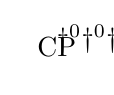
\begin{tikzpicture}[baseline]

        \tikzset{level 1/.style={sibling distance=-80pt}}
        \Tree   [.\node(cp){CP};
                    [.CP$\dag$
                        C$^0$
                        [.TP
                            [.DP$\dag$
                                [.D$^{0}\dag$ she ]
                            ]
                            [.TP$\dag$
                                [.T$^0$ should ]
                                [.VP
                                    [.VP$\dag$
                                        [.V$^0$ bring ]
                                        [.\node(dp){DP};
                                            [.D$^0$ which ]
                                            [.NP
                                                [.N$^0$ flower ]
                                            ]
                                        ]
                                    ]
                                    [.PP
                                        [.P$^0$ here ]
                                    ]
                                ]
                            ]
                        ]
                    ]
                    [.\node(xp){XP};
                        [.X$^0$ Q ]
                        \edge [draw=none]; {}
                    ]
                ]

            \draw [bend left=40] (xp.south) to (dp.north);

    \end{tikzpicture}
\end{exe}

%
%\begin{exe}
%	\exr{ex:multi3}
%	% \small
%	\jtree
%	\! = {CP} <left>[xunit=4.5em]!left ^<right>[xunit=6em]!right .
%	\!left =
%		{CP$\dag$}
%		:[xunit=2.5em]{\obar{C}} [xunit=2.5em]{TP}
%		:[xunit=2.7em]{DP$\dag$}(<vert>{\obar{D}$\dag$}(<vert>{she})) [xunit=2.7em]{TP$\dag$}
%		:[xunit=2.6em]{\obar{T}}(<vert>{should}) [xunit=2.7em]{VP}
%		:[xunit=2.5em]! [xunit=2.9 em]{PP}<vert>{\obar{P}}<vert>{here}
%		.
%		\! = {VP$\dag$}
%		:[xunit=2em]{\obar{V}}(<vert>{bring}) [xunit=2em]{DP}@s
%		:[xunit=1.5em]{\obar{D}}(<vert>{which}) [xunit=1.5em]{NP}<vert>{\obar{N}}<vert>{flower}
%		.
%	\!right =
%		{XP}@r
%		<left>[xunit=2em]{\obar{X}}<vert>{Q}
%		.
%		\nccurve[dirA=(1:-1),dirB=(.8:1)]{-}{r:b}{s:t}
%	\endjtree
%\end{exe}

As we've seen, \emph{which} and \emph{flower} have two paths in (\ref{ex:multi3}), and so the largest $\Pi$ contains them both:
\begin{exe}
	\ex \label{ex:bigpimulti3}
	\begin{xlist}
		\ex $p$(\emph{which}) = \{DP, VP$\dag$, VP, TP$\dag$, TP, CP$\dag$, CP\}
		\ex $p$(\emph{which}) = \{DP, XP, CP\}
		\ex $p$(\emph{flower}) = \{NP, DP, VP$\dag$, VP, TP$\dag$, TP, CP$\dag$, CP\}
		\ex $p$(\emph{flower}) = \{NP, DP, XP, CP\}
		\ex $p$(\emph{bring}) = \{VP$\dag$, VP, TP$\dag$, TP, CP$\dag$, CP\}
		\ex $p$(\emph{here}) = \{PP, VP, TP$\dag$, TP, CP$\dag$, CP\}
		\ex $p$(\emph{should}) = \{TP$\dag$, TP, CP$\dag$, CP\}
		\ex $p$(\emph{she}) = \{DP$\dag$, TP, CP$\dag$, CP\}
		\ex $p$(\emph{Q}) = \{XP, CP\}
	\end{xlist}
\end{exe}

\newpage
The values for $d$ are:
\begin{exe}
	\ex \label{ex:bigdmulti3}
	\begin{xlist}
		\ex $d$(CP) = \{\emph{she}, \emph{should}, \emph{bring}, \emph{here}, \emph{Q}, \emph{which}, \emph{flower}\}
		\ex \label{ex:bdmulti3xp}$d$(XP) = \{\emph{Q}, \emph{which}, \emph{flower}\}
		\ex $d$(CP$\dag$) = \{\emph{she}, \emph{should}, \emph{bring}, \emph{here}, \emph{which}, \emph{flower}\}
		\ex $d$(TP) = \{\emph{she}, \emph{should}, \emph{bring}, \emph{here}, \emph{which}, \emph{flower}\}
		\ex $d$(DP$\dag$) = \{\emph{she}\}
		\ex $d$(TP$\dag$) = \{\emph{should}, \emph{bring}, \emph{here}, \emph{which}, \emph{flower}\}
		\ex \label{ex:vp} $d$(VP) = \{\emph{bring}, \emph{here}, \emph{which}, \emph{flower}\}
		\ex \label{ex:vpdag}$d$(VP$\dag$) = \{\emph{bring}, \emph{which}, \emph{flower}\}
		\ex $d$(DP) = \{\emph{which}, \emph{flower}\}
		\ex $d$(NP) = \{\emph{flower}\}
	\end{xlist}
\end{exe}

(\ref{ex:engine}) prevents almost all linearizations of (\ref{ex:bigpimulti3}). It allows a \isi{linearization} for this $\Pi$ only under very narrow circumstances: when the language's word order settings would allow the multidominant phrase to be simultaneously contiguous to the sisters it has in both of its positions. Because of (\ref{ex:bdmulti3xp}), (\ref{ex:engine}) requires the \isi{linearization} to have a contiguous string made from \emph{Q, which} and \emph{flower}. But because of (\ref{ex:vp}) and (\ref{ex:vpdag}), it also requires contiguous substrings made from \{\emph{bring, which, flower}\} and \{\emph{bring, which, flower, here}\}, which means the \isi{linearization} must have one of the strings in~(\ref{ex:prel}) in~it.
\begin{exe}
	\ex \label{ex:prel}
	\begin{xlist}
		\ex \label{ex:no}
		\begin{xlist}
		\ex bring which flower here
		\ex bring flower which here
		\end{xlist}
		\ex \label{ex:last}
		\begin{xlist}
		\ex here bring which flower
		\ex here bring flower which
		\end{xlist}
		\ex \label{ex:first}
		\begin{xlist}
		\ex which flower bring here
		\ex flower which bring here
		\end{xlist}
	\end{xlist}
\end{exe}

The strings in (\ref{ex:no}) can't coexist in a \isi{linearization} that also puts \emph{Q} contiguous with \{\emph{which, flower}\}. The strings in (\ref{ex:last}) and (\ref{ex:first}) can if nothing in larger phrases separates \emph{Q}. For instance, the strings in~(\ref{ex:samples}) would satisfy~(\ref{ex:engine}).
\begin{exe}
	\ex \label{ex:samples}
	\begin{xlist}
		\ex Q which flower bring here should she
		\ex she should here bring which flower Q
	\end{xlist}
\end{exe}
%
I don't know of such a case, but I don't know of any harm in letting in this possibility. In general, though, (\ref{ex:bigpimulti3}) is too large to have a viable outcome. A smaller $\Pi$ will have to be chosen.

There are four other $\Pi$s that satisfy Totality. They all give to \emph{which} and \emph{flower} just one path. One such $\Pi$ chooses paths for \emph{which} and \emph{flower} that go through XP; another chooses paths for \emph{which} and \emph{flower} that go through VP$\dag$ instead. The first of these is (\ref{ex:overtmulti3}) and the second~(\ref{ex:covertmulti3}).
\begin{exe}
	\ex \label{ex:overtmulti3}
	\begin{xlist}
		\ex $p$(\emph{which}) = \{DP, XP, CP\}
		\ex $p$(\emph{flower}) = \{NP, DP, XP, CP\}
		\ex $p$(\emph{bring}) = \{VP$\dag$, VP, TP$\dag$, TP, CP$\dag$, CP\}
		\ex $p$(\emph{here}) = \{PP, VP, TP$\dag$, TP, CP$\dag$, CP\}
		\ex $p$(\emph{should}) = \{TP$\dag$, TP, CP$\dag$, CP\}
		\ex $p$(\emph{she}) = \{DP$\dag$, TP, CP$\dag$, CP\}
		\ex $p$(\emph{Q}) = \{XP, CP\}
	\end{xlist}
	\ex \label{ex:covertmulti3}
	\begin{xlist}
		\ex $p$(\emph{which}) = \{DP, VP$\dag$, VP, TP$\dag$, TP, CP$\dag$, CP\}
		\ex $p$(\emph{flower}) = \{NP, DP, VP$\dag$, VP, TP$\dag$, TP, CP$\dag$, CP\}
		\ex $p$(\emph{bring}) = \{VP$\dag$, VP, TP$\dag$, TP, CP$\dag$, CP\}
		\ex $p$(\emph{here}) = \{PP, VP, TP$\dag$, TP, CP$\dag$, CP\}
		\ex $p$(\emph{should}) = \{TP$\dag$, TP, CP$\dag$, CP\}
		\ex $p$(\emph{she}) = \{DP$\dag$, TP, CP$\dag$, CP\}
		\ex $p$(\emph{Q}) = \{XP, CP\}
	\end{xlist}
\end{exe}

The $d$s for (\ref{ex:overtmulti3}) are in (\ref{ex:overtdmulti3}), and they correspond to the string in~(\ref{ex:overtstringmulti3}) in a head-initial and Specifier-initial language like English.
\begin{exe}
	\ex \label{ex:overtdmulti3}
	\begin{xlist}
		\ex $d$(CP) = \{\emph{she}, \emph{should}, \emph{bring}, \emph{here}, \emph{Q}, \emph{which}, \emph{flower}\}
		\ex $d$(XP) = \{\emph{Q}, \emph{which}, \emph{flower}\}
		\ex $d$(CP$\dag$) = \{\emph{she}, \emph{should}, \emph{bring}, \emph{here}\}
		\ex $d$(TP) = \{\emph{she}, \emph{should}, \emph{bring}, \emph{here}\}
		\ex $d$(DP$\dag$) = \{\emph{she}\}
		\ex $d$(TP$\dag$) = \{\emph{should}, \emph{bring}, \emph{here}\}
		\ex $d$(VP) = \{\emph{bring}, \emph{here}\}
		\ex $d$(VP$\dag$) = \{\emph{bring}\}
		\ex $d$(DP) = \{\emph{which}, \emph{flower}\}
		\ex $d$(NP) = \{\emph{flower}\}
	\end{xlist}
		\ex \label{ex:overtstringmulti3} Q which flower she should bring here
\end{exe}

The $d$s for (\ref{ex:covertmulti3}) are in (\ref{ex:covertdmulti3}), and they correspond to the string in~(\ref{ex:covertstringmulti3}), in a head-initial, Specifier-initial language.
\begin{exe}
	\ex \label{ex:covertdmulti3}
	\begin{xlist}
		\ex $d$(CP) = \{\emph{she}, \emph{should}, \emph{bring}, \emph{here}, \emph{Q}, \emph{which}, \emph{flower}\}
		\ex $d$(XP) = \{\emph{Q}\}
		\ex $d$(CP$\dag$) = \{\emph{she}, \emph{should}, \emph{bring}, \emph{here}, \emph{which}, \emph{flower}\}
		\ex $d$(TP) = \{\emph{she}, \emph{should}, \emph{bring}, \emph{here}, \emph{which}, \emph{flower}\}
		\ex $d$(DP$\dag$) = \{\emph{she}\}
		\ex $d$(TP$\dag$) = \{\emph{should}, \emph{bring}, \emph{here}, \emph{which}, \emph{flower}\}
		\ex $d$(VP) = \{\emph{bring}, \emph{here}, \emph{which}, \emph{flower}\}
		\ex $d$(VP$\dag$) = \{\emph{bring}, \emph{which}, \emph{flower}\}
		\ex $d$(DP) = \{\emph{which}, \emph{flower}\}
		\ex $d$(NP) = \{\emph{flower}\}
	\end{xlist}
	\ex \label{ex:covertstringmulti3} Q she should bring which flower
\end{exe}

These are the desired outcomes; they correspond to the overt and covert \isi{movement} possibilities.

The remaining two $\Pi$s that satisfy Totality give to \emph{which} and
\emph{flower} divergent paths. They are both blocked by the \gls{PCA}. To see
how, consider (\ref{ex:divergent}), where \emph{flower} is given a path through
XP and \emph{which} is given a path through~VP$\dag$.%\largerpage[3]

%The remaining two $\Pi$s that satisfy Totality give to \emph{which} and
%\emph{flower} divergent paths. Both are blocked by the \gls{PCA}. To see
%how, consider (\ref{ex:divergent}): \emph{flower} is given a path through
%XP and \emph{which} is given a path through~VP$\dag$. The \emph{d}s for
%(\ref{ex:divergent}) are~(\ref{ex:divergentd}).

\begin{exe}
	\ex \label{ex:divergent}
	\begin{xlist}
		\ex $p$(\emph{which}) = \{DP, VP$\dag$, VP, TP$\dag$, TP, CP$\dag$, CP\}
		\ex $p$(\emph{flower}) = \{NP, DP, XP, CP\}
		\ex $p$(\emph{bring}) = \{VP$\dag$, VP, TP$\dag$, TP, CP$\dag$, CP\}
		\ex $p$(\emph{here}) = \{PP, VP, TP$\dag$, TP, CP$\dag$, CP\}
		\ex $p$(\emph{should}) = \{TP$\dag$, TP, CP$\dag$, CP\}
		\ex $p$(\emph{she}) = \{DP$\dag$, TP, CP$\dag$, CP\}
		\ex $p$(\emph{Q}) = \{XP, CP\}
	\end{xlist}
\end{exe}
The \emph{d}s for (\ref{ex:divergent}) are~(\ref{ex:divergentd}).
\begin{exe}
	\ex \label{ex:divergentd}
	\begin{xlist}
		\ex $d$(CP) = \{\emph{she}, \emph{should}, \emph{bring}, \emph{here}, \emph{Q}, \emph{which}, \emph{flower}\}
		\ex $d$(XP) = \{\emph{Q}, \emph{flower}\}
		\ex $d$(CP$\dag$) = \{\emph{she}, \emph{should}, \emph{bring}, \emph{here}, \emph{which}\}
		\ex $d$(TP) = \{\emph{she}, \emph{should}, \emph{bring}, \emph{here}, \emph{which}\}
		\ex $d$(DP$\dag$) = \{\emph{she}\}
		\ex $d$(TP$\dag$) = \{\emph{should}, \emph{bring}, \emph{here}, \emph{which}\}
		\ex $d$(VP) = \{\emph{bring}, \emph{here}, \emph{which}\}
		\ex $d$(VP$\dag$) = \{\emph{bring}, \emph{which}\}
		\ex $d$(DP) = \{\emph{which}, \emph{flower}\}
		\ex $d$(NP) = \{\emph{flower}\}
	\end{xlist}
\end{exe}

$d$(VP$\dag$) and $d$(VP) together require that the \isi{linearization} produce the
string \emph{bring which here} (once English-specific choices are made). But
$d$(DP) requires that the \isi{linearization} also produce the string \emph{which
flower}. There is no way of linearizing these words that preserves these two
requirements. Exactly the same incompatibility arises if the path for
\emph{flower} goes through VP$\dag$ and the path for \emph{which} goes through
XP -- the other way of choosing divergent paths for these words. The reason
these choices lead to a conflict is because all choices of paths for
\emph{which} and \emph{flower} will contain DP, and (\ref{ex:engine}) will
consequently require \emph{which} and \emph{flower} to be contiguous. This is
how this system prevents the words in a moved phrase from getting linearized in
different positions.

The \gls{PCA}, then, allows for both overt and covert \isi{movement} and, like the
\gls{MLCA}, explains why multidominant structures allow for selective
relaxation of Contiguity. It makes Contiguity, rather than asymmetric
c-command, the driving force behind a \isi{linearization}. The formalization of
Contiguity involved enforces a particular kind of ``nesting'' condition on
entire phrase markers\is{phrase marker}. It allows \isi{multidominance} in just those cases where that
nesting condition can be satisfied for every word in the \isi{phrase marker} without
considering the complete structure of the sentence.

% section paths (end)

\section{Summary} % (fold)
\label{sec:30.summary}

What I've shown here is a way of completing Nunes' method of deriving Terseness
that involves defining the ``copy of α'' as ``giving α an addition position in
the \isi{phrase marker}.'' Traditional \isi{linearization} schemes have stood in the
way of such a move. I've offered two new \isi{linearization} algorithms that
don't, each with slightly different empirical footprints.



\printchapterglossary{}

\section*{Acknowledgements}

This paper is largely a channeling of many people's thoughts. These include
Sakshi Bhatia, David Erschler, Hsin-Lun Huang, Rodica Ivan, Jyoti Iyer, Petr
Kusily, Deniz Ozyildiz, Ethan Poole, Katia Vostrikova, Michael Wilson, Rong
Yin, Rajesh Bhatt, Peggy Speas, Nikolaos Angelopoulos, John Gluckman, Nicoletta
Loccioni, Travis Major, Iara Mantenuto, Sozen Ozkan, Richard Stockwell, Carson
Schutze and Tim Hunter. A special thanks to Leland Kusmer whose guidance has
improved this paper in many ways.

{\sloppy
\printbibliography[heading=subbibliography,notkeyword=this]
}

\end{document}
